

\begin{figure}
\centering
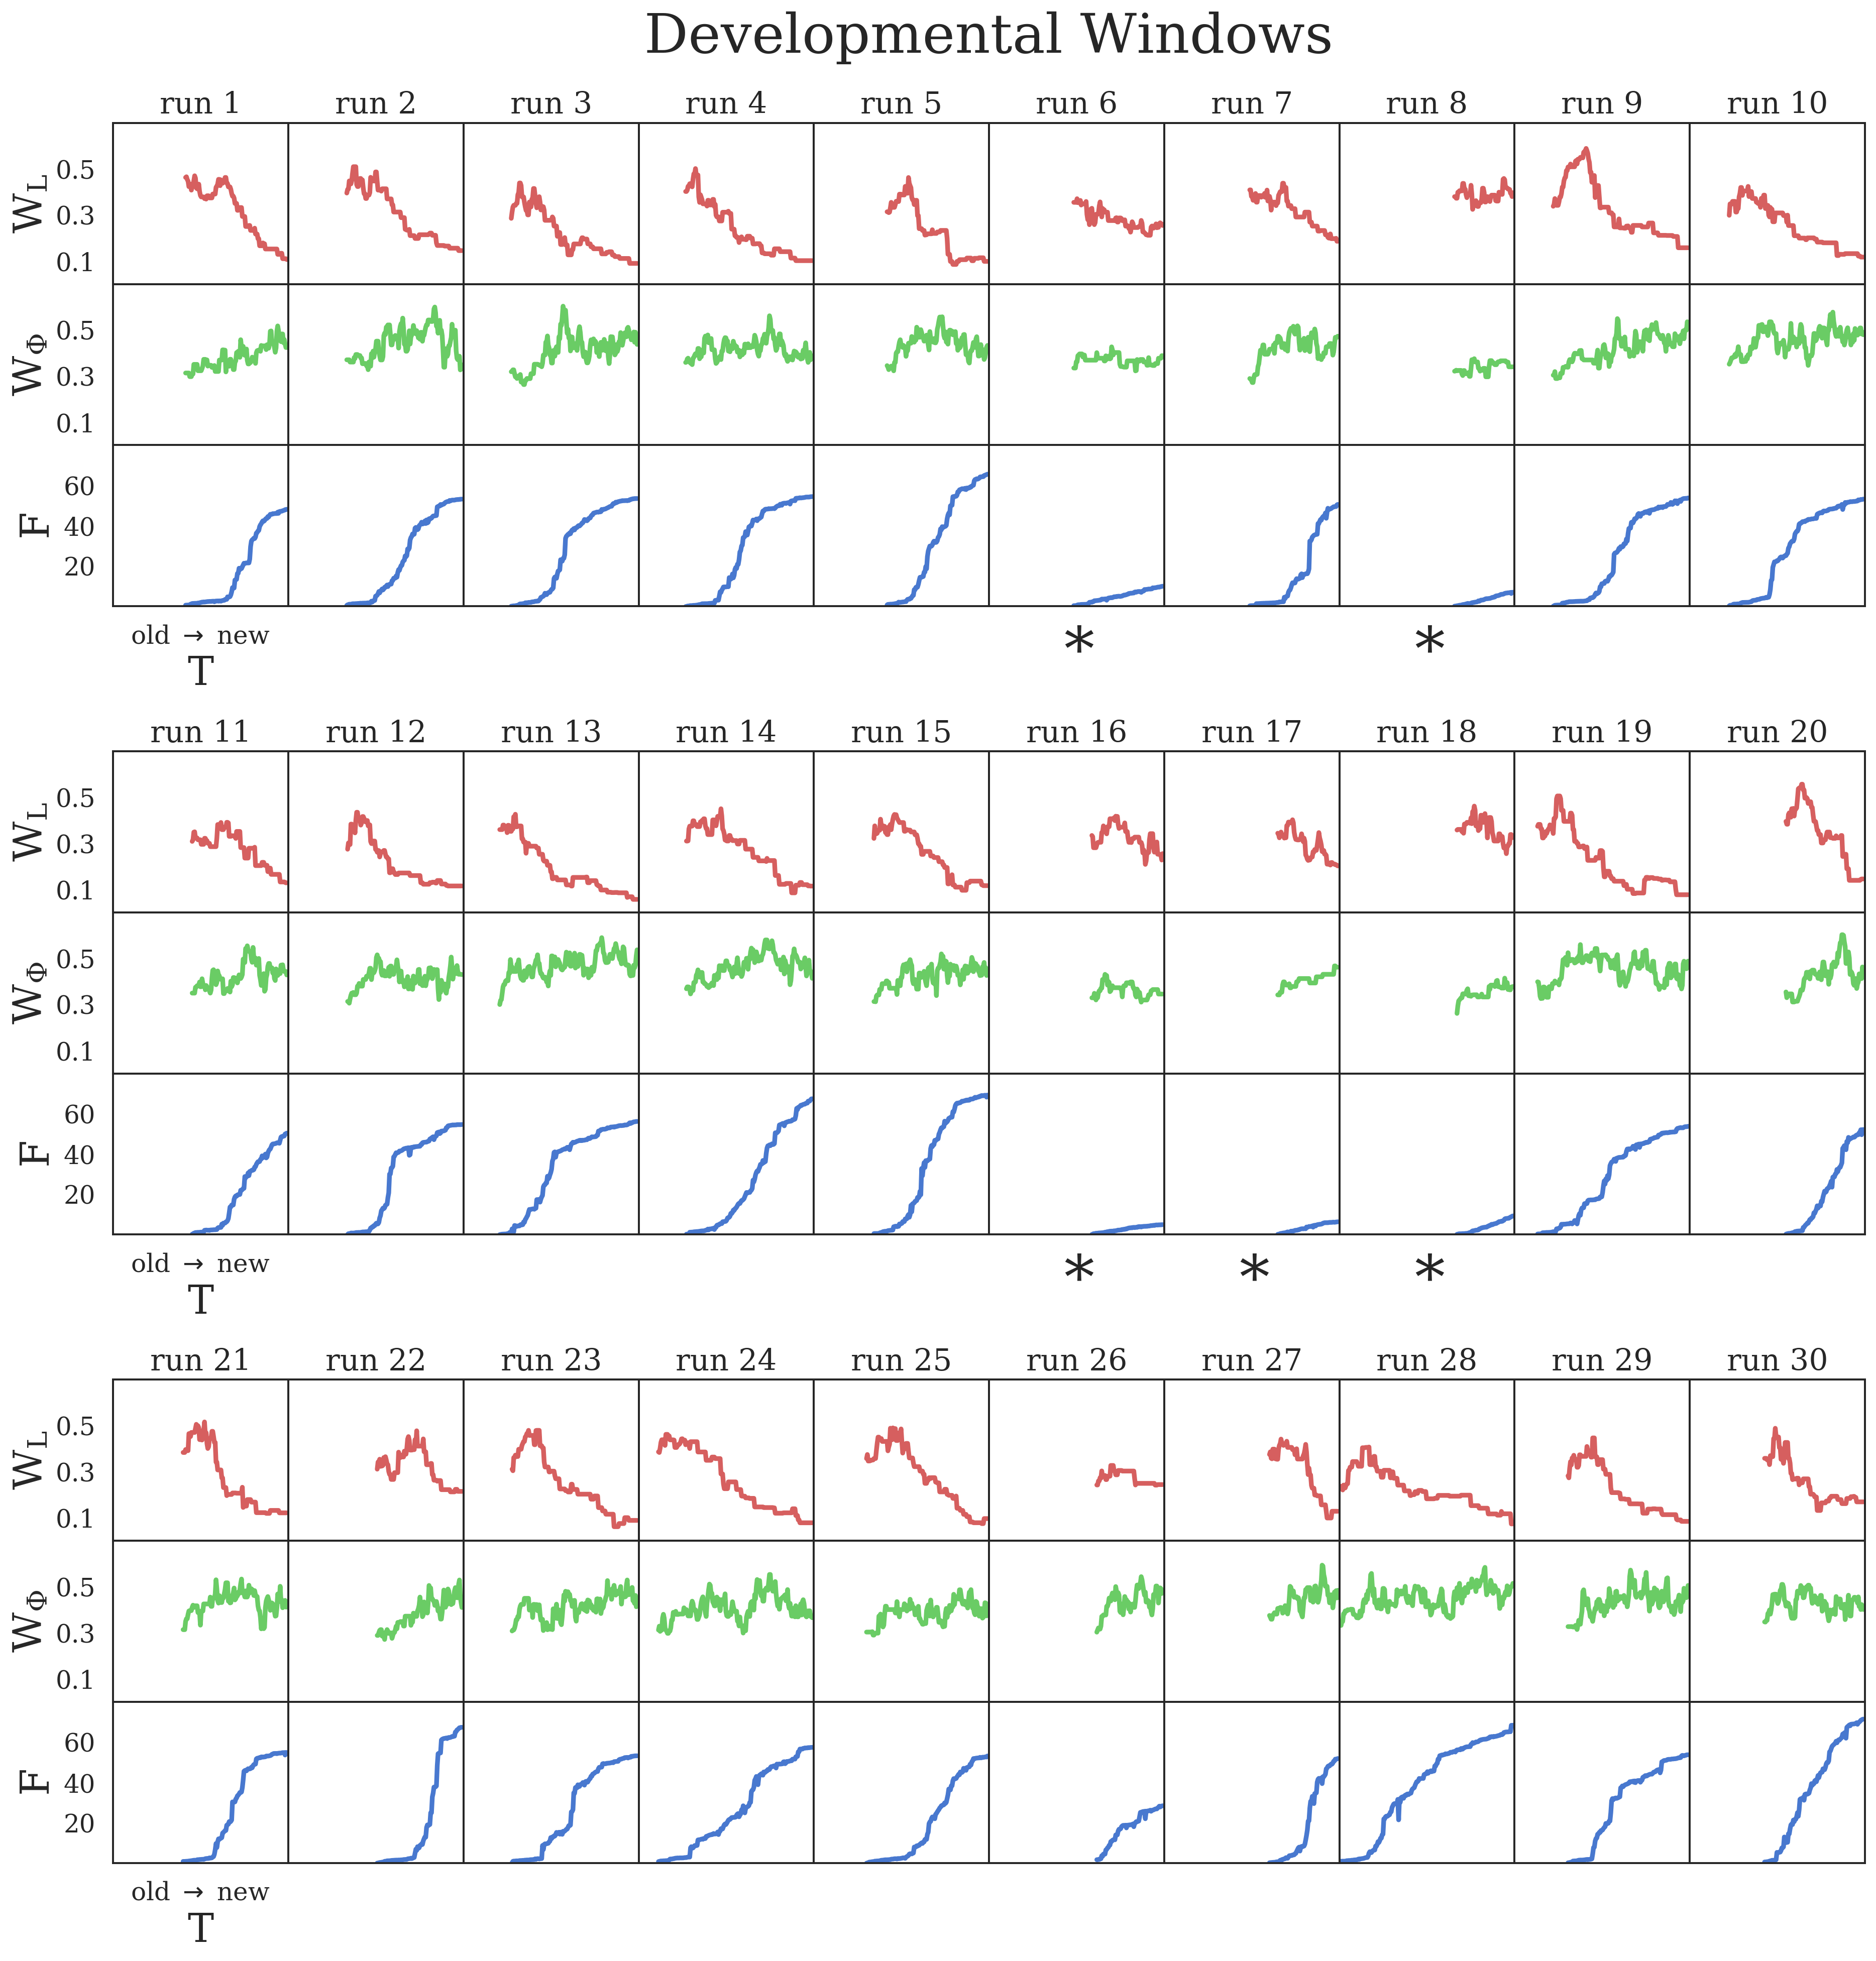
\includegraphics[width=\linewidth]{Chapter04/FigS1}
\caption{\label{fig:S1}\textbf{Evolutionary change during 30 Evo-Devo trials.} The amount of morphological development, $W_L$ (see Equation 3), controller development, $W_{\Phi}$ (see Equation 4), and fitness, $F$, for the lineages of the 30 Evo-Devo run champions. Evolutionary time, $T$, moves from the oldest ancestor (left) to the run champion (right). A general trend emerges wherein lineages initially increase their morphological development in $T$ (rising red curves) and subsequently decrease morphological development to almost zero (falling red curves). Five of the 30 evolutionary trials, annotated by {\Large $\ast$}, fell into a local optima.}
\end{figure}



\begin{figure}
\centering
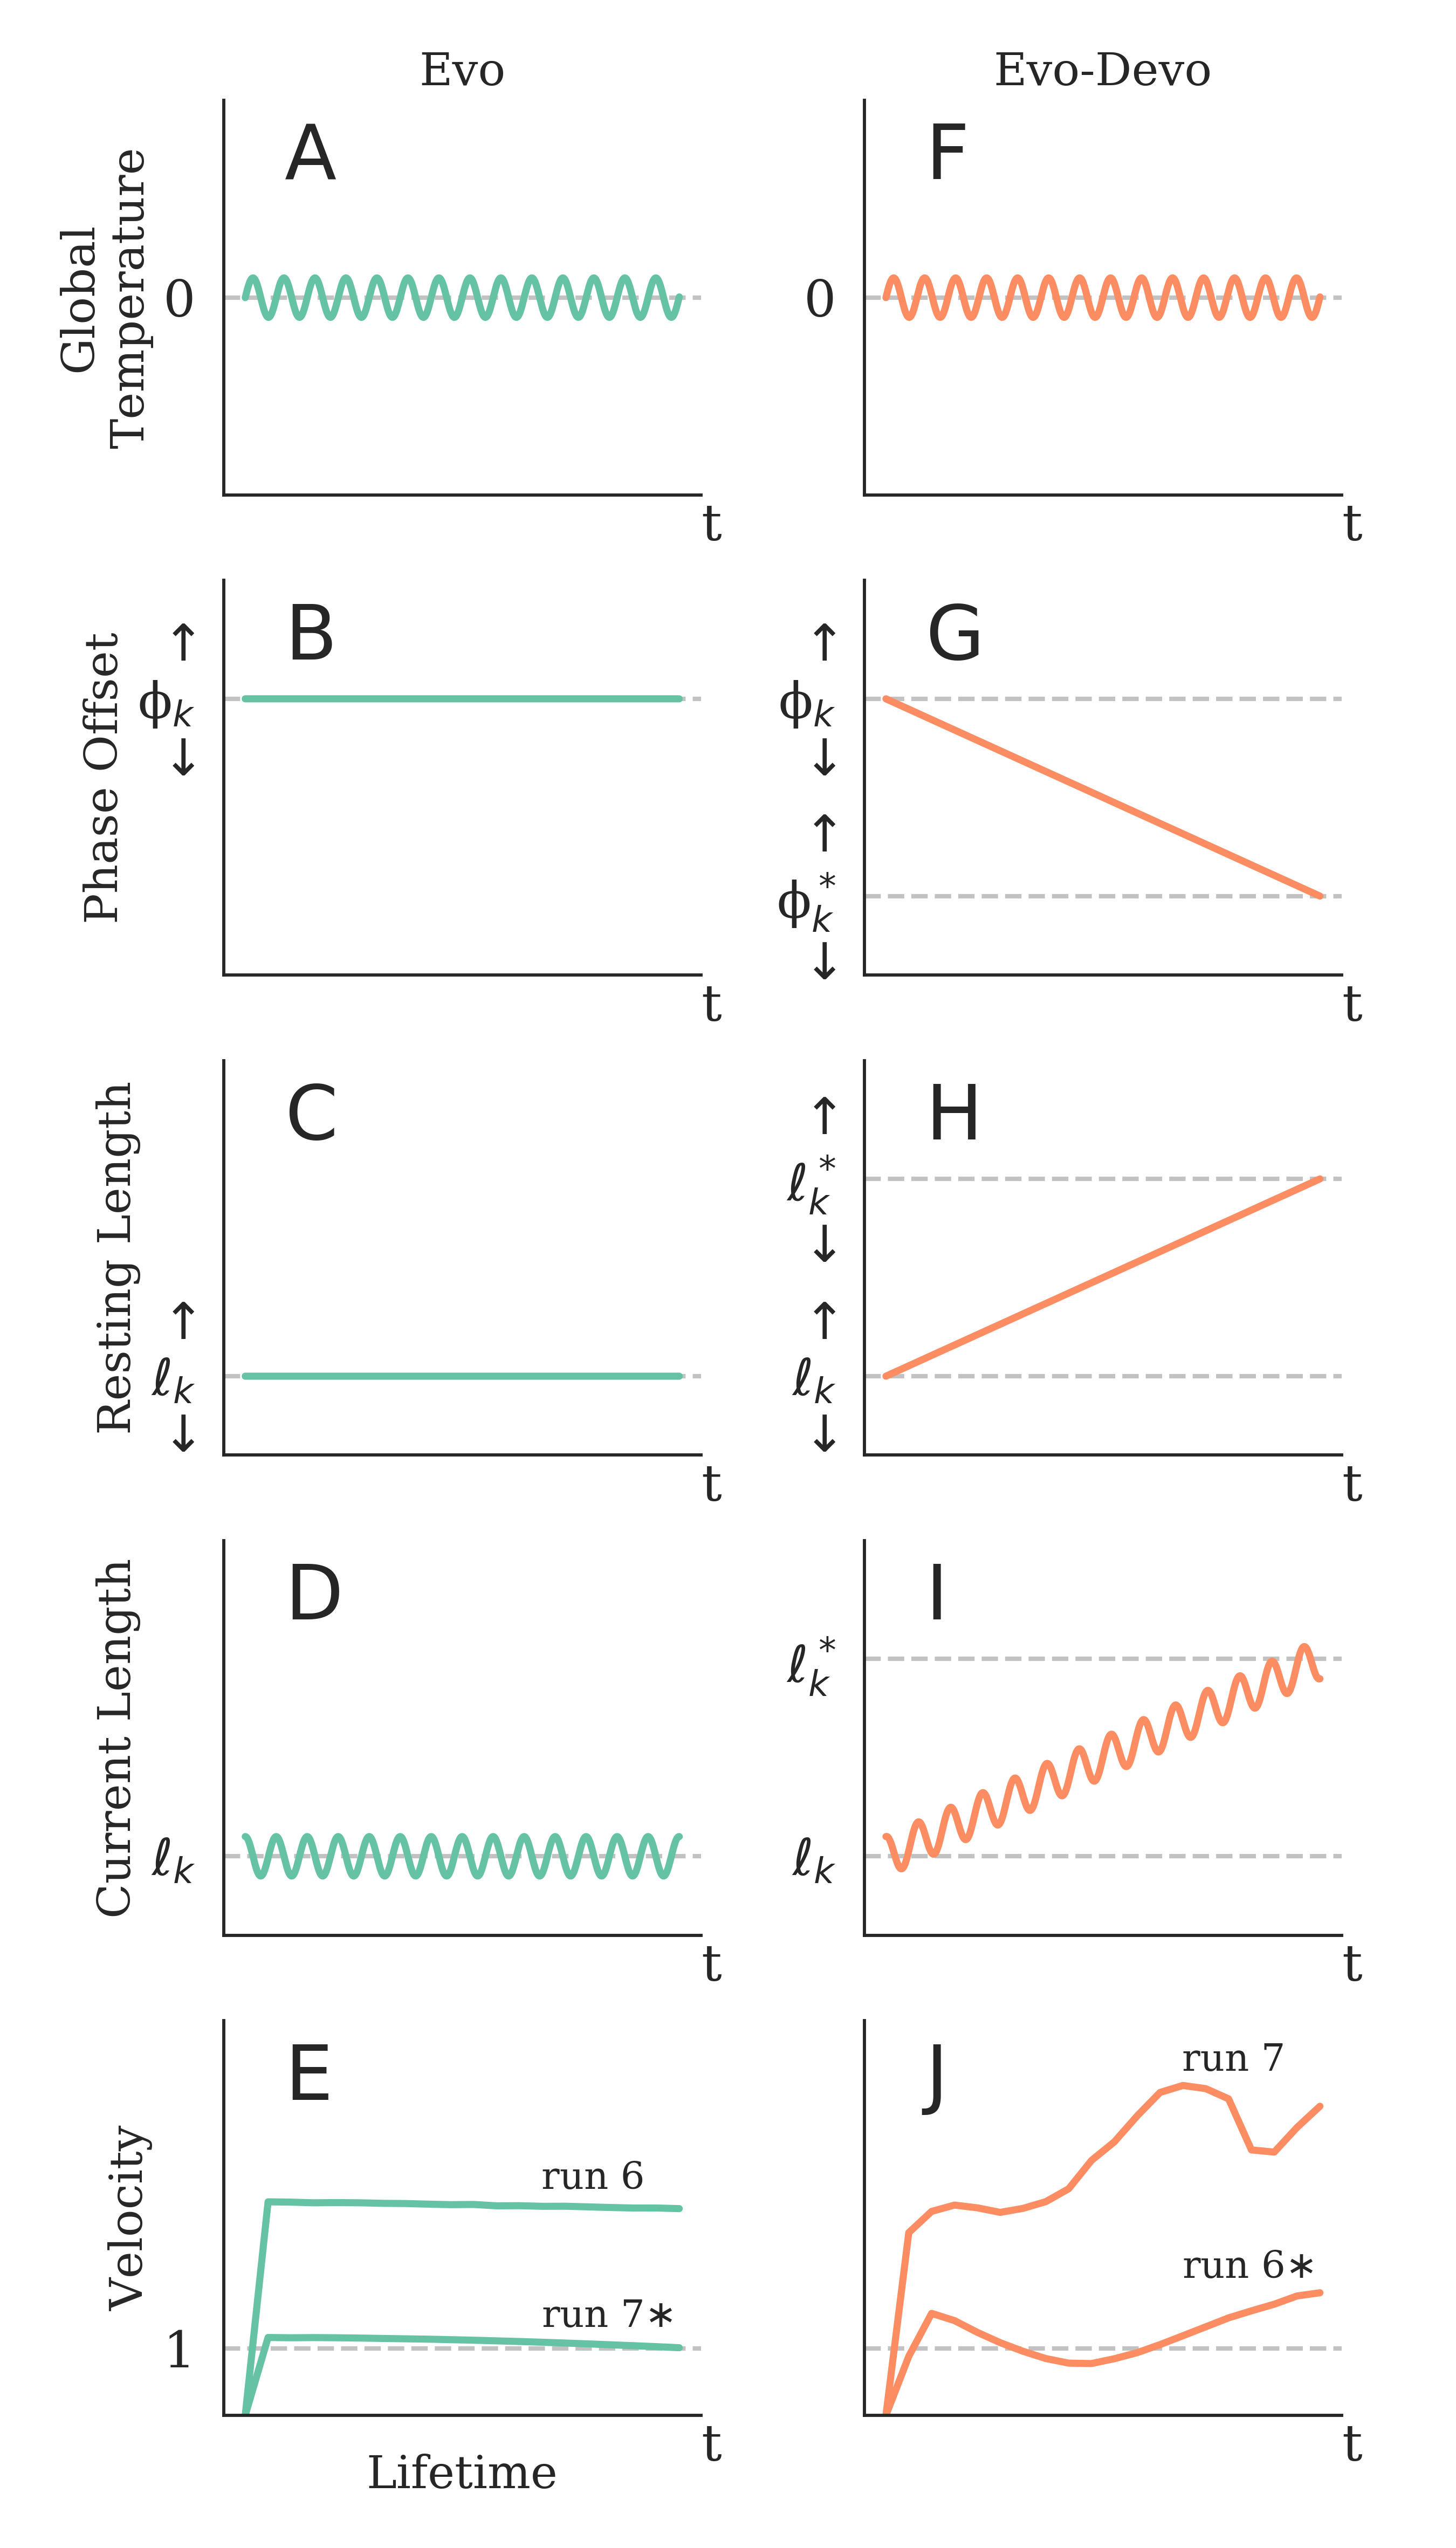
\includegraphics[width=0.6\linewidth]{Chapter04/FigS2}
\vspace{-4pt}
\caption{\label{fig:S2}\textbf{Experimental treatments.} The phase of an oscillating global temperature (A, F) is offset in the $k$-th voxel by a linear function from $\phi_k$ to $\phi_k^*$ (B, G). 
The resting length of the $k$-th voxel is a linear function from $\ell_k$ to $\ell_k^*$ (C, H). 
For Evo, there is no development, so $\phi_k=\phi_k^*$ and $\ell_k=\ell_k^*$.
The offset actuation is added on top of the resting length to give the current length of the $k$-th voxel (D, I). 
These example voxel-level changes occur across ontogenetic time $(t)$, independently in each of the 48 voxels, and together interact with the environment to generate robot-level velocity (E, J).
To see this, we averaged displacement across intervals of two actuation cycles (0.5 sec) and plotted the smoothed velocities for two Evo-Devo run champions with minimal canalization (J) alongside their non-developmental counterparts (E).
Also note that the frequency of actuation is plotted here at 1.4 Hz; but, in our experiments, we used a frequency of 4 Hz.
}
\end{figure}




\begin{figure}
\centering
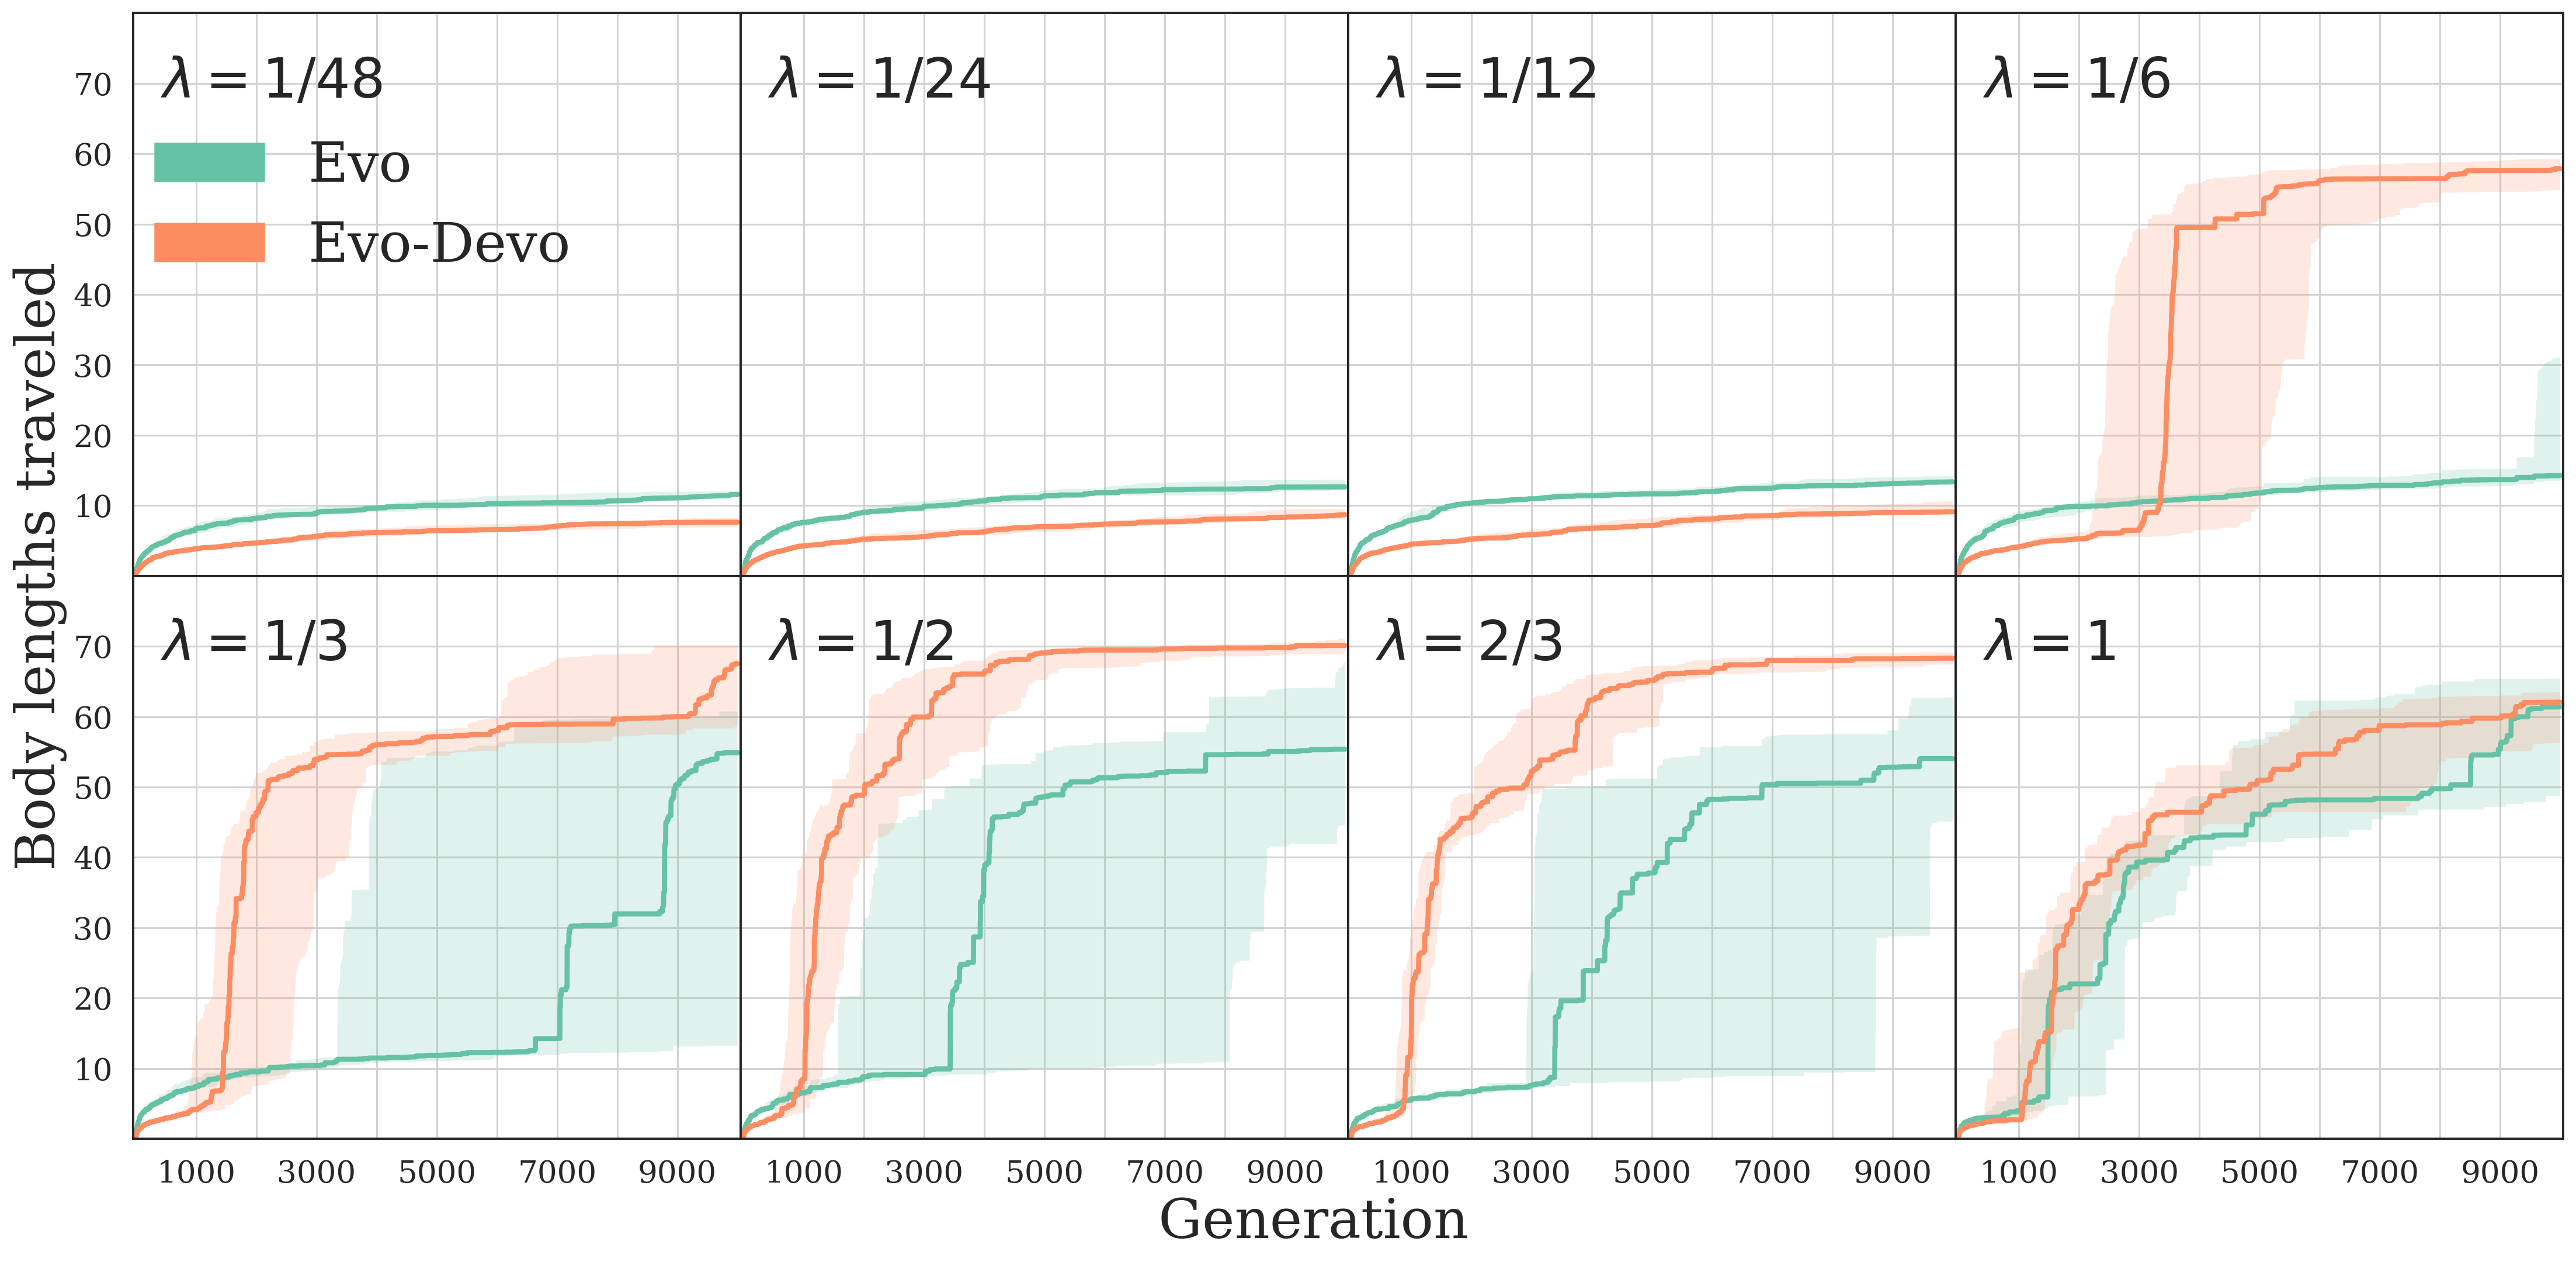
\includegraphics[width=\linewidth]{Chapter04/FigS3}
\caption{\label{fig:S3}\textbf{Mutation rate sweep.} 
Median fitness (with 95\% bootstrapped confidence intervals) under various mutation rates, $\lambda$, a hyperparameter defined in Supplementary Methods which affects the probability a voxel is mutated. 
In the main experiment of this paper, the mutation rate is evolved for each voxel independently, and is constantly changing.
In this mutation rate sweep, $\lambda$ is held uniform across all voxels.
There were two observed basins of attraction in terms of fitness: a slower design that trots/gallops 5-15 body-lengths during the evaluation period, and a faster design type that rolls at 50-70 body-lengths. 
Although higher mutation rates facilitate the discovery of the superior phenotype, once found, lower mutation rates tend to produce more refined and faster robots.
Without development, the search space has a single spike of high fitness. 
One can not do better than random search in such a space.
When $\lambda=1$, optimizing Evo morphologies reduces to random search, and this is the only mutation rate where Evo does not require significantly more generations than Evo-Devo to find the faster design type.
This can be observed for $\lambda\in\{1/6,\, 1/3,\, 1/2,\, 2/3,\, 1\}$, by comparing the generation at which the slopes of the fitness curves increase dramatically.
However, the best two treatments (Evo-Devo at $\lambda=1/2$ and $\lambda=2/3$), as measured by the highest median speed at the end of optimization, have development, and the robots they produced are significantly faster than those produced by random search (Evo with the highest mutation rate)
$(p<0.01)$.
}
\end{figure}



\begin{figure}
\centering
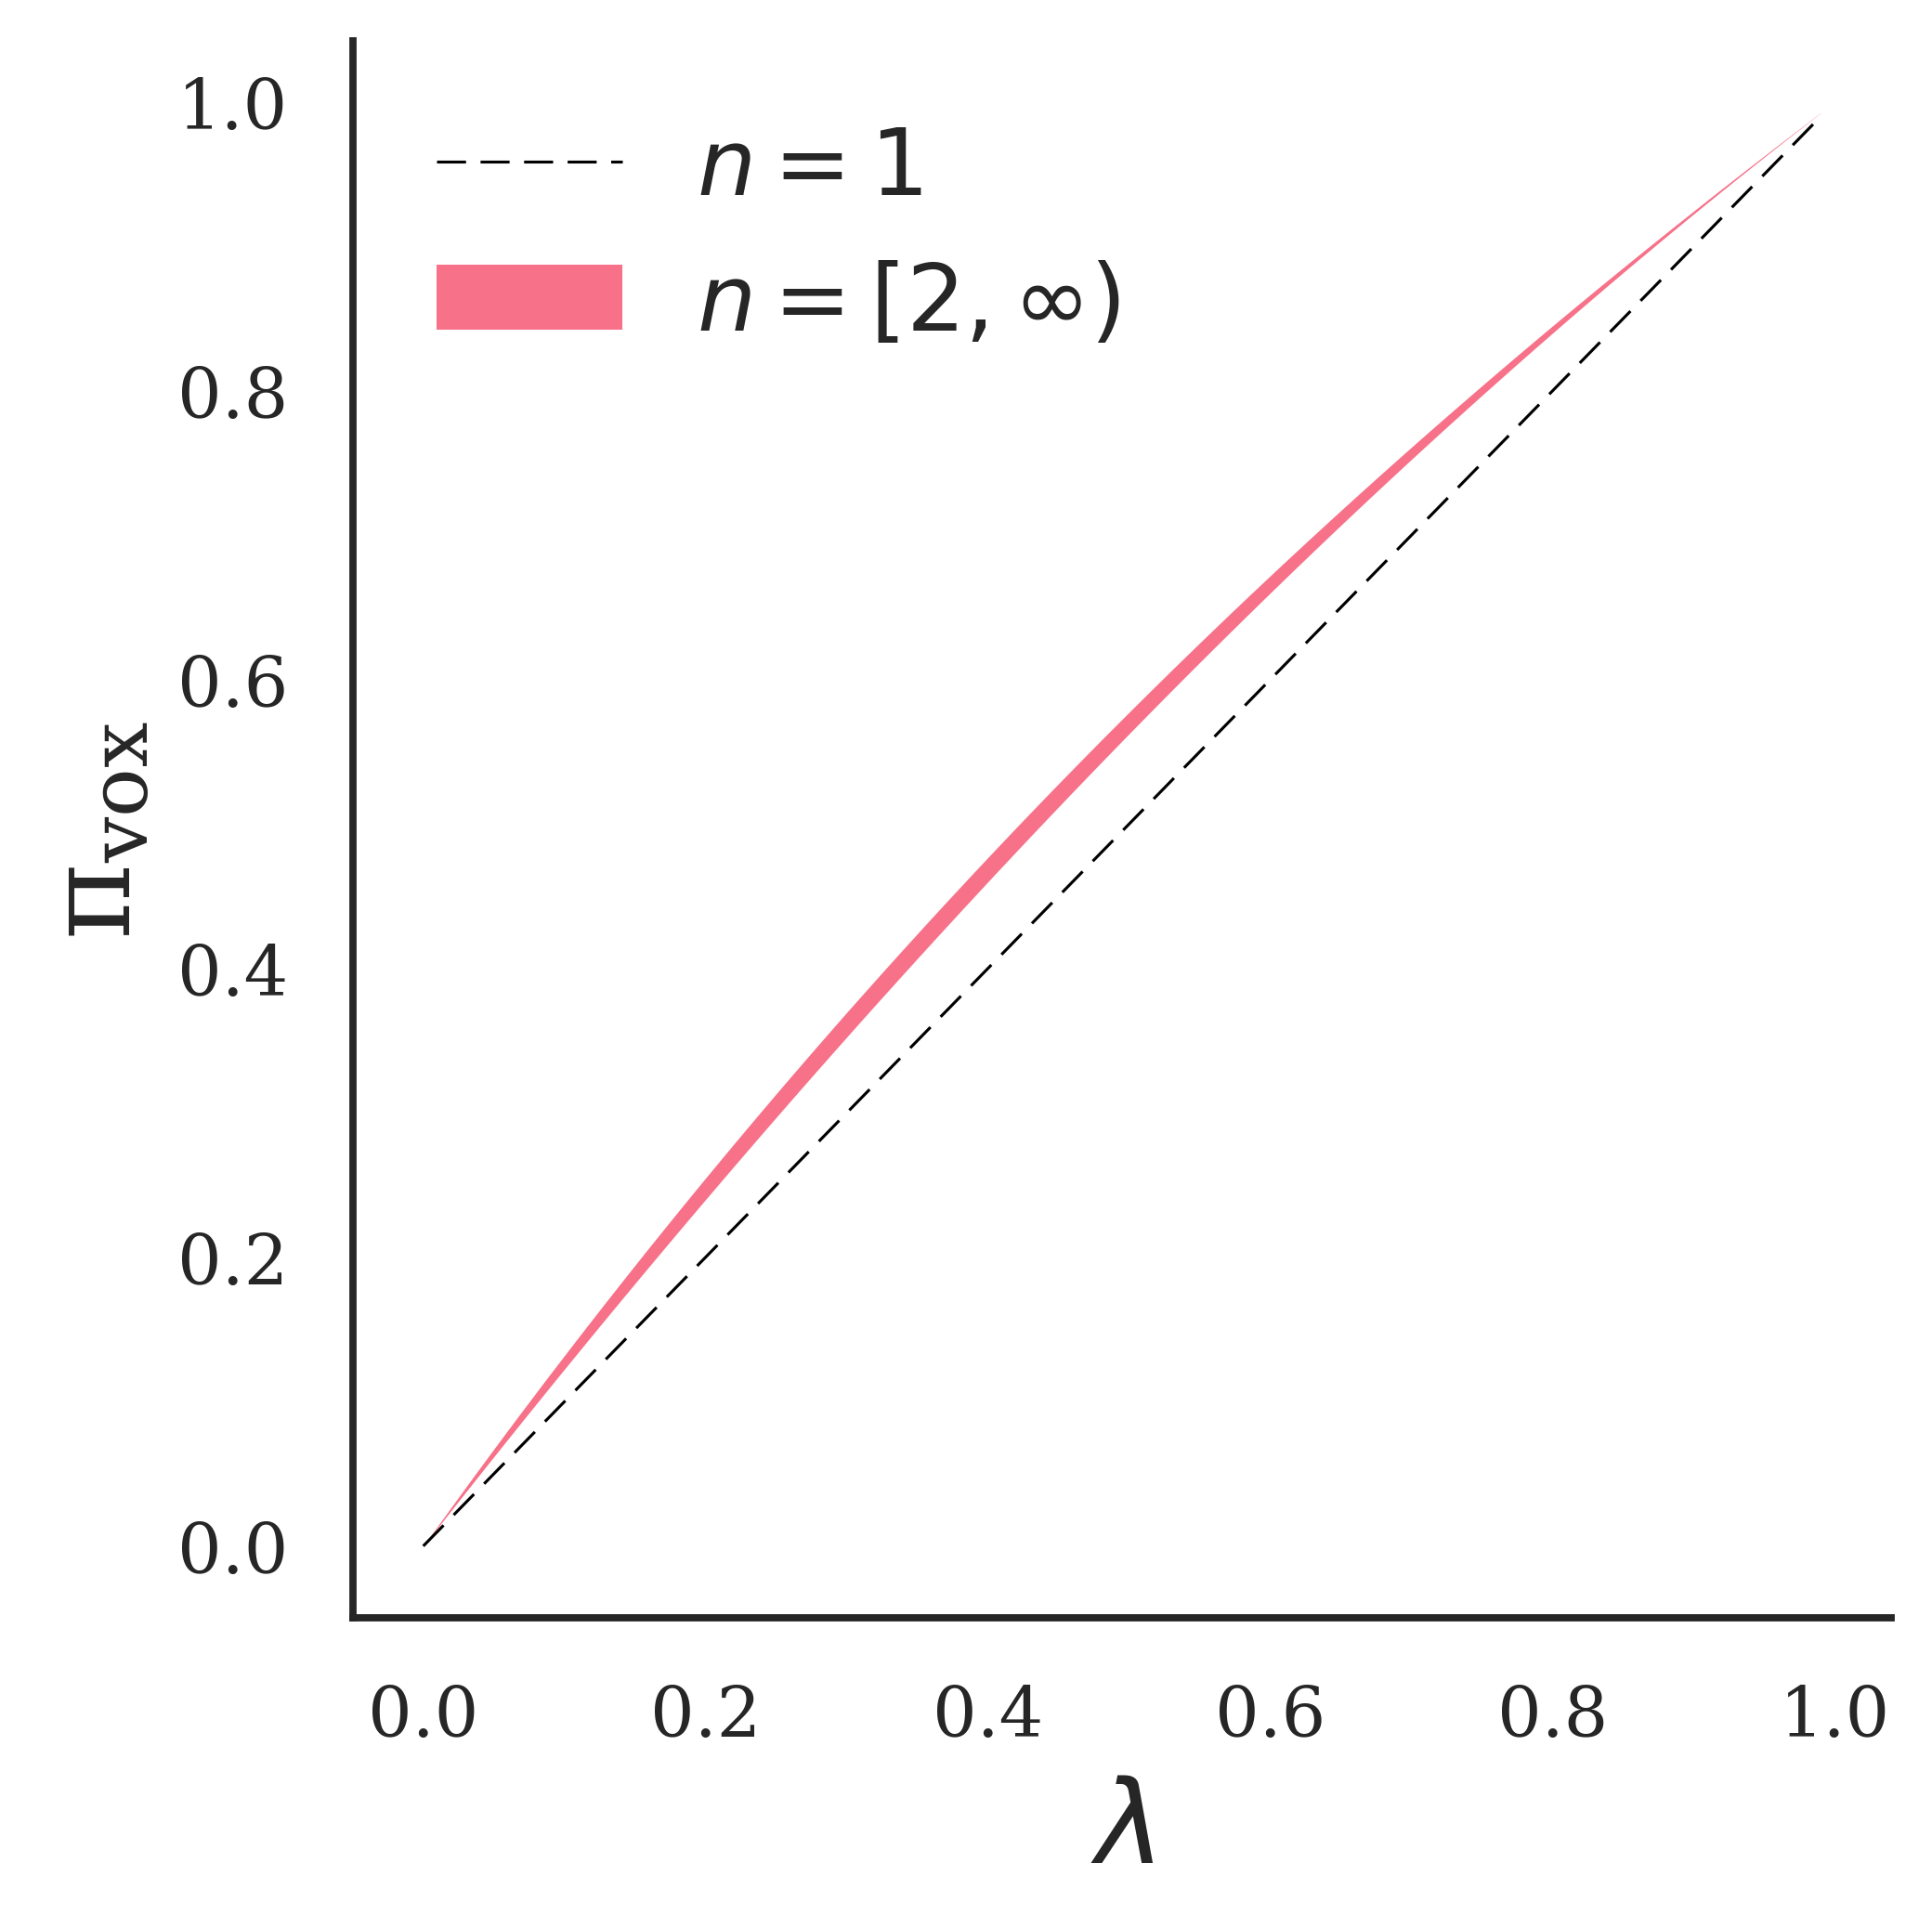
\includegraphics[width=0.5\linewidth]{Chapter04/FigS4}
\caption{\label{fig:S4}\textbf{Mutational impact.} The expected proportion of voxels modified, $\pi_{\text{vox}}$, where $n$ is the number of material properties that can be mutated, and $\lambda$ is the mutation rate.
A derivation is provided in Supplementary Methods.
Regardless of $n$,
when $\lambda=1$, every voxel must be mutated, and when $\lambda=0$, no voxels can be mutated. 
Between these two points, there is an extremely tight bound on the proportion of voxels mutated for any $n>1$. 
In this paper, we have treatments Evo, with $n=2$, and Evo-Devo, with $n=4$.
}
\end{figure}




\begin{figure}
\centering
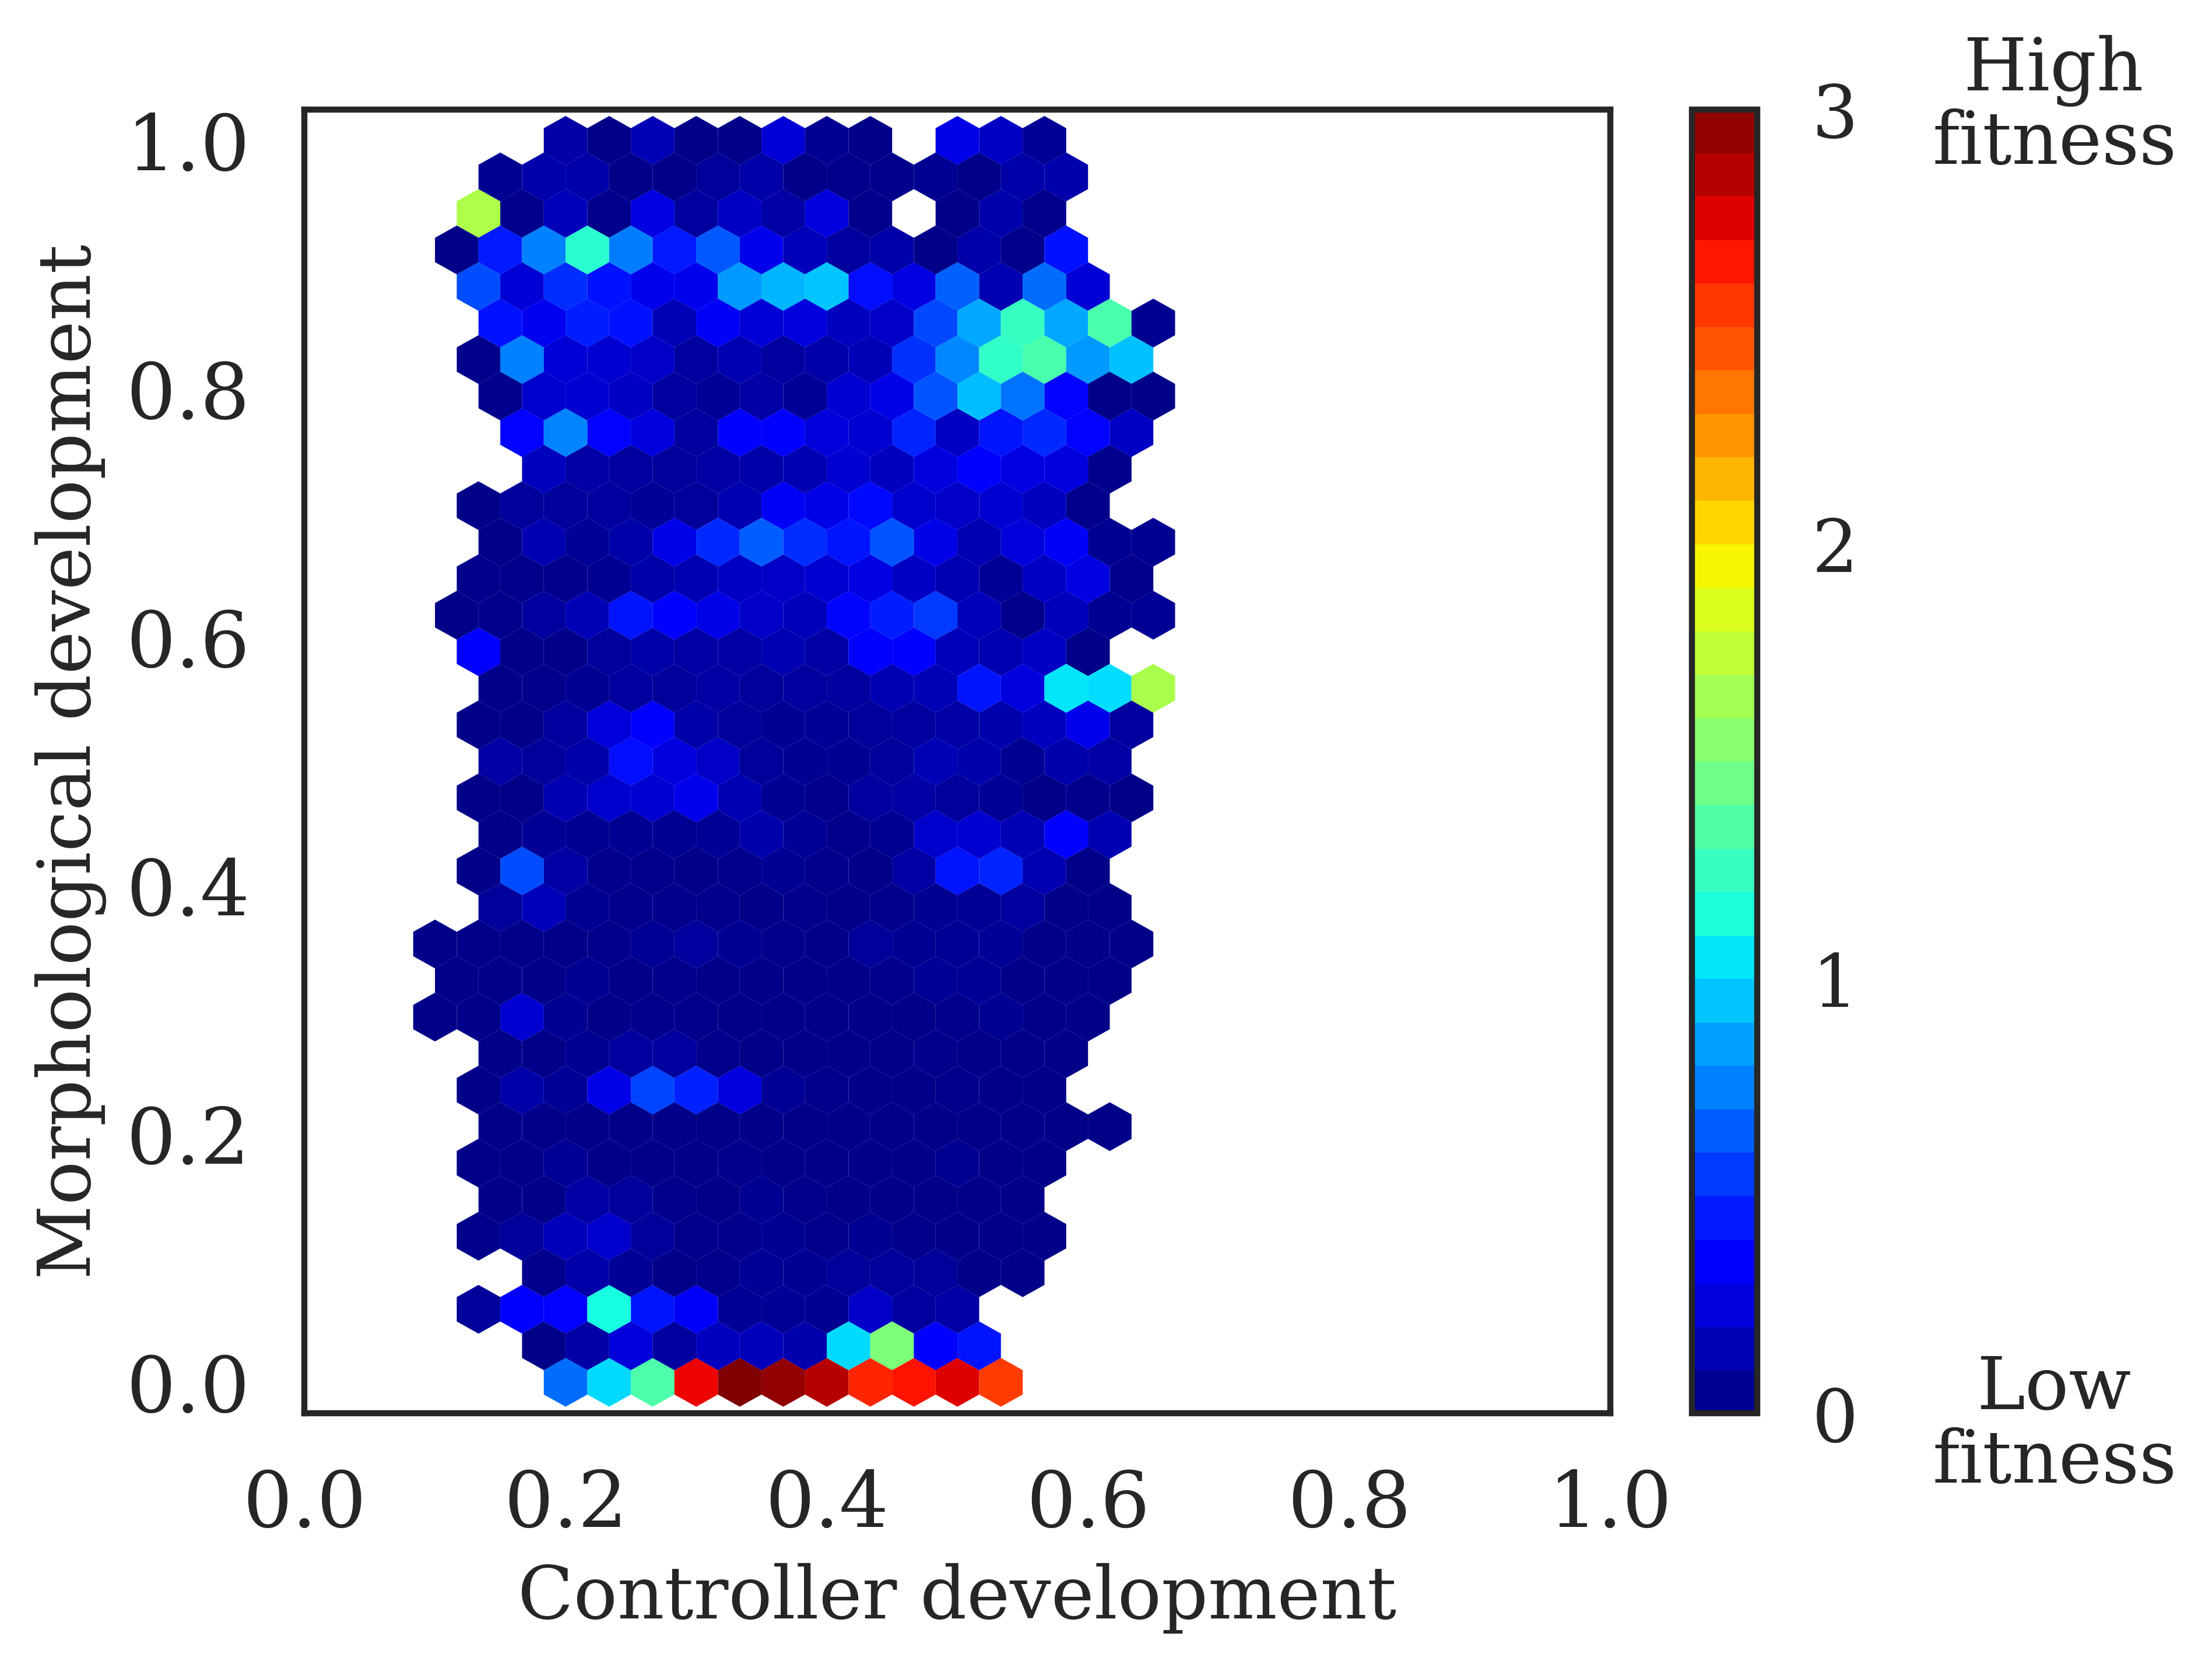
\includegraphics[width=0.65\linewidth]{Chapter04/FigS5}
\caption{\label{fig:S5}\textbf{Differential canalization in rigid bodies.} 
This environment consists of a sloped floor, declined toward a light source. 
Rigid-bodied robots, which are described in Supplementary Methods, perform phototaxis.
Although longer legs produce faster walking behaviors, the shortest leg setting places the robot's large, spherical abdomen onto the ground, allowing the robot to simply roll down the ramp toward the light. 
An ancestor discovers rolling over toward the end of its evaluation period through ontogenetic morphological change that compresses leg lengths. 
This rollable morphology is assimilated to the start of development through differential canalization: The sooner a robot shrinks its legs, the sooner it can begin rolling; eventually descendants start with compressed legs, are able to immediately roll, exhibit little to no morphological change, but continue to sweep over many different synaptic weights as they behave. 
Rolling down the slope is not entirely passive, however, since protruding legs, even at their shortest setting, can slow down or even stop forward movement. 
The best controllers not only avoid such interference, but also guide rolling toward the light source. 
However, development in this particular case did not affect evolvability. 
These results are consistent with predictions made by other quantitative models used in theoretical biology that suggest that plasticity only expedites evolution under restrictive conditions \cite{ancel2000undermining}. 
We hypothesize that, in our case, this is because the search space is not deceptive enough: Once the rigid-bodied robot evolves to compress its legs, and touch its abdomen to the sloped floor, it will tend to roll for the remainder of its evaluation period.
That is, in contrast with the soft robots, there is no intermediate stage between walking and rolling that suffers the fitness penalty of no longer being able to move.
}
\end{figure}





